% 第0章 排版示例：一本书里能写出什么
% 这是给撰写人看的示例章，正式出版前可以整章删除。
\documentclass[../../main.tex]{subfiles}

\begin{document}

% 让本章编号为 0，后面各章仍从 1 开始编号
\setcounter{chapter}{-1}

\chapter{排版示例：一本书里能写出什么}
\label{ch:00-guide}

这一章是给撰写人看的\textbf{示例章}：把书里能用的写法一层一层演示一遍。每处都是先给"写法"、
再给"效果"，写正文时照着抄就行。正式出版前整章删除即可。

\begin{itemize}
  \item 第 \ref{sec:00-structure} 节：章、节、小节的层级
  \item 第 \ref{sec:00-text} 节：文字格式　第 \ref{sec:00-lists} 节：列表
  \item 第 \ref{sec:00-tables} 节：表格　第 \ref{sec:00-pictures} 节：图片
  \item 第 \ref{sec:00-math} 节：公式与定理　第 \ref{sec:00-source} 节：代码
  \item 第 \ref{sec:00-crossref} 节：交叉引用与文献　第 \ref{sec:00-boxes} 节：提示框
  \item 第 \ref{sec:00-details} 节：排版细节　第 \ref{sec:00-assets} 节：素材放哪里
\end{itemize}

\section{章、节、小节的层级}
\label{sec:00-structure}

书的结构只有三层：\textbf{章}（\verb|\chapter|）→ \textbf{节}（\verb|\section|）→
\textbf{小节}（\verb|\subsection|）。章标题写在每章的 \texttt{chapter.tex} 里，
节和小节写在各自的小节文件里。编号和目录都是自动生成的，不用手写"第一节""1.1"这种编号。

写法：

\begin{lstlisting}[language=TeX]
\section{章、节、小节的层级}
\label{sec:00-structure}          % 标签供交叉引用使用，见第 0.8 节

\subsection{这是小节（二级标题）}
\label{sec:00-structure-sub}

\subsubsection{这是更小的一级（三级标题）}
\end{lstlisting}

效果：本节标题和下面这两级，就是你正在看的效果。

\subsection{这是小节（二级标题）}
\label{sec:00-structure-sub}

小节下面是正文段落。正文照常用中文写就行，段首缩进、行距、中西文间距都是自动排的。

\subsubsection{这是更小的一级（三级标题）}

一般不建议再往下分。层级太深，读者反而看不清结构。

\KeyPoint{关于 \texttt{\textbackslash label} 的命名}{约定是"类型:章-节-序号"，
例如 \texttt{sec:04-processor-core-02}、\texttt{fig:04-pipeline-stages}、
\texttt{tab:00-comparison}。标签名里不要用中文，也不要用空格。}

\begin{lstlisting}[language=TeX]
\subsection{这是小节（二级标题）}
这是正文。段落之间空一行，LaTeX 会自动缩进。

不要在源码里手动加空格或空行来"凑"排版效果——那是自动排的。
\end{lstlisting}

\section{文字格式}
\label{sec:00-text}

常用的文字格式都在下面这张对照里，左边是效果，右边是写法。

\begin{description}
  \item[加粗] \verb|\textbf{加粗}| → \textbf{加粗}；正文强调用加粗，不要用下划线
  \item[斜体] \verb|\emph{斜体}| 或 \verb|\textit{斜体}| → \emph{斜体}
  \item[等宽] \verb|\texttt{main.tex}| → \texttt{main.tex}
  \item[下划线] \verb|\underline{下划线}| → \underline{下划线}（慎用，容易和链接混淆）
  \item[彩色] \verb|\textcolor{Accent}{强调色}| → \textcolor{Accent}{强调色}
  \item[大一号/小一号] \verb|\large 大一点|、\verb|\small 小一点| →
    {\large 大一点}、{\small 小一点}
  \item[脚注] \verb|\footnote{补充说明}| → 见页脚\footnote{这就是脚注的样子，
    适合放不打断正文的补充说明。}
  \item[行内代码] \texttt{\textbackslash verb|make -j8|} → \verb|make -j8|
  \item[链接] \verb|\url{https://example.com}| → \url{https://example.com}
  \item[带文字的链接] \verb|\href{https://example.com}{点这里}| →
    \href{https://example.com}{点这里}
\end{description}

中文标点直接用键盘输入的全角符号就行：，。；：？！""''（）《》——……
中西文之间的空隙由排版引擎自动处理，\textbf{不要手动敲空格}。

\begin{lstlisting}[language=TeX]
这段话里有\textbf{加粗}、\emph{斜体}和\texttt{等宽}，
还有一条脚注\footnote{脚注内容}。
\end{lstlisting}

效果：

这段话里有\textbf{加粗}、\emph{斜体}和\texttt{等宽}，还有一条脚注\footnote{脚注内容}。

\KeyPoint{写作建议}{一段话只讲一件事，超过五行就拆成两段。技术名词第一次出现时
给全称和缩写，例如"指令集架构（Instruction Set Architecture, ISA）"。}

\section{列表}
\label{sec:00-lists}

\subsection{无序列表与嵌套}

写法：

\begin{lstlisting}[language=TeX]
\begin{itemize}
  \item 第一点
  \item 第二点
    \begin{itemize}
      \item 需要展开时再嵌一层
      \item 一般不要超过两层
    \end{itemize}
\end{itemize}
\end{lstlisting}

效果：

\begin{itemize}
  \item 第一点
  \item 第二点
    \begin{itemize}
      \item 需要展开时再嵌一层
      \item 一般不要超过两层
    \end{itemize}
\end{itemize}

\subsection{有序列表}

\begin{lstlisting}[language=TeX]
\begin{enumerate}
  \item 先装 TeX Live
  \item 再编译：\verb|scripts/build.sh|
  \item 最后检查 \texttt{build/main.log}
\end{enumerate}
\end{lstlisting}

效果：

\begin{enumerate}
  \item 先装 TeX Live
  \item 再编译：\verb|scripts/build.sh|
  \item 最后检查 \texttt{build/main.log}
\end{enumerate}

需要从指定编号开始时，写成 \verb|\begin{enumerate}[start=3]|。

\subsection{术语对照列表}

定义型的对照用 \texttt{description}，术语加粗放在方括号里：

\begin{lstlisting}[language=TeX]
\begin{description}
  \item[ISA] 指令集架构，软件与硬件之间的契约。
  \item[SoC] 片上系统，把处理器核、外设、存储器接口集成在一颗芯片上。
\end{description}
\end{lstlisting}

效果：

\begin{description}
  \item[ISA] 指令集架构，软件与硬件之间的契约。
  \item[SoC] 片上系统，把处理器核、外设、存储器接口集成在一颗芯片上。
\end{description}

\subsection{实验验收清单}

每节的实验都建议给一份可以逐项打勾的清单，用数学符号做方框：

\begin{lstlisting}[language=TeX]
\begin{itemize}
  \item[$\square$] 编译通过，没有错误
  \item[$\boxtimes$] 波形符合预期
\end{itemize}
\end{lstlisting}

效果：

\begin{itemize}
  \item[$\square$] 编译通过，没有错误
  \item[$\boxtimes$] 波形符合预期
\end{itemize}

\section{表格}
\label{sec:00-tables}

\subsection{三线表（最常用）}

教材里的表格一律用三线表：上下各一条粗线，表头下面一条细线，中间不画竖线。

写法：

\begin{lstlisting}[language=TeX]
\begin{table}[htbp]
\centering
\caption{三种处理器对比}
\label{tab:00-compare}
\begin{tabular}{@{}lll@{}}
\toprule
项目 & 单周期 & 五级流水线 \\
\midrule
指令吞吐 & 1 条/周期 & 最高 1 条/周期（重叠执行）\\
关键路径 & 长，主频低 & 短，主频高 \\
实现难度 & 低 & 需要处理冒险 \\
\bottomrule
\end{tabular}
\end{table}
\end{lstlisting}

效果：

\begin{table}[htbp]
\centering
\caption{三种处理器对比}
\label{tab:00-compare}
\begin{tabular}{@{}lll@{}}
\toprule
项目 & 单周期 & 五级流水线 \\
\midrule
指令吞吐 & 1 条/周期 & 最高 1 条/周期（重叠执行）\\
关键路径 & 长，主频低 & 短，主频高 \\
实现难度 & 低 & 需要处理冒险 \\
\bottomrule
\end{tabular}
\end{table}

\subsection{自动换行的宽表}

单元格文字长、又要占满版心时，用 \texttt{tabularx} 配 \texttt{Y} 列（自动换行、
左对齐）或 \texttt{P\{宽度\}} 列：

\begin{lstlisting}[language=TeX]
\begin{table}[htbp]
\centering
\caption{接口信号说明}
\label{tab:00-signals}
\begin{tabularx}{\linewidth}{@{}P{22mm}Y@{}}
\toprule
信号 & 说明 \\
\midrule
\texttt{clk} & 时钟，上升沿有效；所有时序逻辑都在它的上升沿更新 \\
\texttt{rst\_n} & 异步复位，低电平有效；复位后取指地址回到启动地址 \\
\bottomrule
\end{tabularx}
\end{table}
\end{lstlisting}

效果：

\begin{table}[htbp]
\centering
\caption{接口信号说明}
\label{tab:00-signals}
\begin{tabularx}{\linewidth}{@{}P{22mm}Y@{}}
\toprule
信号 & 说明 \\
\midrule
\texttt{clk} & 时钟，上升沿有效；所有时序逻辑都在它的上升沿更新 \\
\texttt{rst\_n} & 异步复位，低电平有效；复位后取指地址回到启动地址 \\
\bottomrule
\end{tabularx}
\end{table}

\subsection{合并单元格与对齐}

\begin{lstlisting}[language=TeX]
\begin{table}[htbp]
\centering
\caption{合并表头与按列对齐}
\label{tab:00-merged}
\begin{tabular}{@{}llrr@{}}
\toprule
批次 & 类型 & \multicolumn{2}{c}{耗时 / ns} \\
\cmidrule(lr){3-4}
     &      & 典型 & 最差 \\
\midrule
\multirow{2}{*}{A} & 译码 & 1.2 & 1.5 \\
                   & 执行 & 2.0 & 2.8 \\
\bottomrule
\end{tabular}
\end{table}
\end{lstlisting}

效果（数字列用 \texttt{r} 右对齐，读起来整齐）：

\begin{table}[htbp]
\centering
\caption{合并表头与按列对齐}
\label{tab:00-merged}
\begin{tabular}{@{}llrr@{}}
\toprule
批次 & 类型 & \multicolumn{2}{c}{耗时 / ns} \\
\cmidrule(lr){3-4}
     &      & 典型 & 最差 \\
\midrule
\multirow{2}{*}{A} & 译码 & 1.2 & 1.5 \\
                   & 执行 & 2.0 & 2.8 \\
\bottomrule
\end{tabular}
\end{table}

\subsection{跨页长表格}

表格超过一页时用 \texttt{longtable}，它会自动在断页处重复表头。写法把
\texttt{table} 换成 \texttt{longtable} 即可，标题放在第一行用
\verb|\caption{...}\\| 给出。本示例只有三行，就不强行断页了。

\KeyPoint{表格的规矩}{表题在\textbf{表的上方}，图题在\textbf{图的下方}；
表格里的数字按小数点对齐（用右对齐列）；单位写在表头里（如"耗时 / ns"），
不要每个格子重复写。}

\section{图片}
\label{sec:00-pictures}

\subsection{一张图}

写法：

\begin{lstlisting}[language=TeX]
\begin{figure}[htbp]
\centering
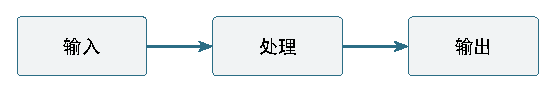
\includegraphics[width=.7\linewidth]{figures/05-pictures/demo-flow}
\caption{数据流示意}
\label{fig:00-flow}
\end{figure}
\end{lstlisting}

效果：

\begin{figure}[htbp]
\centering
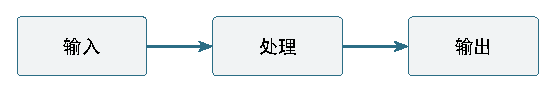
\includegraphics[width=.7\linewidth]{figures/05-pictures/demo-flow}
\caption{数据流示意}
\label{fig:00-flow}
\end{figure}

宽度用 \verb|width=.7\linewidth| 表示"占版心的 70\%"；写成
\verb|width=\linewidth| 就是占满。加 \verb|keepaspectratio| 可以保证不变形
（默认按比例缩放，通常不需要）。

\subsection{两张图并排}

并排用 \texttt{minipage} 左右各占一半，各自带图题：

\begin{lstlisting}[language=TeX]
\begin{figure}[htbp]
\centering
\begin{minipage}{.48\linewidth}
  \centering
  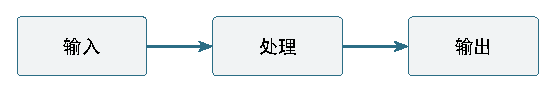
\includegraphics[width=\linewidth]{figures/05-pictures/demo-flow}
  \caption{左图：数据流}
  \label{fig:00-left}
\end{minipage}\hfill
\begin{minipage}{.48\linewidth}
  \centering
  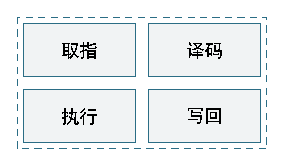
\includegraphics[width=\linewidth]{figures/05-pictures/demo-blocks}
  \caption{右图：阶段划分}
  \label{fig:00-right}
\end{minipage}
\end{figure}
\end{lstlisting}

效果：

\begin{figure}[htbp]
\centering
\begin{minipage}{.48\linewidth}
  \centering
  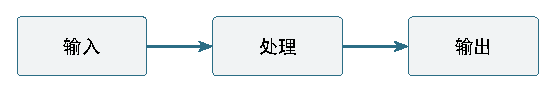
\includegraphics[width=\linewidth]{figures/05-pictures/demo-flow}
  \caption{左图：数据流}
  \label{fig:00-left}
\end{minipage}\hfill
\begin{minipage}{.48\linewidth}
  \centering
  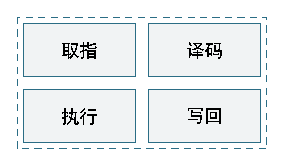
\includegraphics[width=\linewidth]{figures/05-pictures/demo-blocks}
  \caption{右图：阶段划分}
  \label{fig:00-right}
\end{minipage}
\end{figure}

左图是\cref{fig:00-left}，右图是\cref{fig:00-right}——引用时自动带编号。

注意这两张图不一定排在这一段旁边：\textbf{图和表都会浮动}，会被排到页面上更合适的
位置。正因为如此，正文里要写"见\cref{fig:00-left}"，不要写"如下图"。

\subsection{直接用代码画的图}

简单的框图和时序示意其实不必存成图片文件，用 TikZ 直接画在正文里，改起来更快：

\begin{lstlisting}[language=TeX]
\begin{tikzpicture}[box/.style={draw=Accent,fill=Brand!6,rounded corners=2pt,
  minimum width=20mm,minimum height=9mm,align=center,font=\sffamily\small}]
\node[box] (a) {取指};
\node[box,right=8mm of a] (b) {执行};
\draw[->,thick,Accent] (a) -- (b);
\end{tikzpicture}
\end{lstlisting}

效果：

\begin{center}
\begin{tikzpicture}[box/.style={draw=Accent,fill=Brand!6,rounded corners=2pt,
  minimum width=20mm,minimum height=9mm,align=center,font=\sffamily\small}]
\node[box] (a) {取指};
\node[box,right=8mm of a] (b) {执行};
\draw[->,thick,Accent] (a) -- (b);
\end{tikzpicture}
\end{center}

\KeyPoint{选哪种}{需要精确标注的电路图、结构图，用 TikZ 画（矢量、可改）；
截图、相机拍的照片、扫描件，存成图片文件放本章的 \texttt{figures/} 下。
图片文件的命名用小写英文加连字符，例如 \texttt{pipeline-hazard.pdf}。}

\section{公式、定理与例题}
\label{sec:00-math}

\subsection{行内公式与行间公式}

\begin{lstlisting}[language=TeX]
流水线的加速比约为 $S=\dfrac{n}{k+n-1}$，其中 $n$ 是指令条数，$k$ 是流水级数。

\[
  T_{\text{流水}} = \max_i t_i + (n-1)\cdot \max_i t_i
\]
\end{lstlisting}

效果：流水线的加速比约为 $S=\dfrac{n}{k+n-1}$，其中 $n$ 是指令条数，$k$ 是流水级数。

\[
  T_{\text{流水}} = \max_i t_i + (n-1)\cdot \max_i t_i
\]

行内公式前面不要留空行，\verb|$...$| 里的内容也不要换行。

\subsection{带编号、可引用的公式}

\begin{lstlisting}[language=TeX]
\begin{equation}
  \label{eq:00-speedup}
  S = \frac{T_{\text{串行}}}{T_{\text{流水}}}
\end{equation}
\end{lstlisting}

效果：

\begin{equation}
  \label{eq:00-speedup}
  S = \frac{T_{\text{串行}}}{T_{\text{流水}}}
\end{equation}

引用时写 \verb|\cref{eq:00-speedup}|，效果是\cref{eq:00-speedup}。需要换行对齐的
多行公式用 \texttt{align}：

\begin{lstlisting}[language=TeX]
\begin{align}
  S &= \frac{1}{1-p+\frac{p}{k}} \\
    &= \frac{k}{k+(1-p)k} \quad (\text{理想情况})
\end{align}
\end{lstlisting}

效果：

\begin{align}
  S &= \frac{1}{1-p+\frac{p}{k}} \\
    &= \frac{k}{k+(1-p)k} \quad (\text{理想情况})
\end{align}

\subsection{矩阵与分段函数}

\begin{lstlisting}[language=TeX]
\[
  A = \begin{pmatrix} a_{11} & a_{12} \\ a_{21} & a_{22} \end{pmatrix}
  \qquad
  |x| = \begin{cases}
    x,  & x \ge 0 \\
    -x, & x < 0
  \end{cases}
\]
\end{lstlisting}

\[
  A = \begin{pmatrix} a_{11} & a_{12} \\ a_{21} & a_{22} \end{pmatrix}
  \qquad
  |x| = \begin{cases}
    x,  & x \ge 0 \\
    -x, & x < 0
  \end{cases}
\]

\subsection{常用符号}

\begin{center}
\begin{tabular}{@{}llll@{}}
\toprule
写法 & 效果 & 写法 & 效果 \\
\midrule
\verb|\alpha, \beta, \theta| & $\alpha,\beta,\theta$ &
\verb|\sum_{i=1}^{n}| & $\sum_{i=1}^{n}$ \\
\verb|\int_0^T| & $\int_0^T$ &
\verb|\sqrt{x}| & $\sqrt{x}$ \\
\verb|\frac{a}{b}| & $\frac{a}{b}$ &
\verb|\cdot|、\verb|\times| & $\cdot$、$\times$ \\
\verb|\le|、\verb|\ge|、\verb|\ne| & $\le$、$\ge$、$\ne$ &
\verb|\in|、\verb|\subset| & $\in$、$\subset$ \\
\verb|\mathbb{R}| & $\mathbb{R}$ &
\verb|\mathcal{F}| & $\mathcal{F}$ \\
\bottomrule
\end{tabular}
\end{center}

\subsection{定义、定理、例题}

书里已经预置了三种环境，直接用：

\begin{lstlisting}[language=TeX]
\begin{definition}[指令集架构]
软件与硬件之间的契约，规定了可见的寄存器、指令语义、数据类型与异常行为；
它不规定这些行为由怎样的电路实现。
\end{definition}

\begin{theorem}[加速比上界]
在理想流水线下，加速比不超过流水级数 $k$。
\end{theorem}

\begin{example}
一条 5 级流水线，流水线填满后每周期完成 1 条指令。
\end{example}
\end{lstlisting}

效果：

\begin{definition}[指令集架构]
软件与硬件之间的契约，规定了可见的寄存器、指令语义、数据类型与异常行为；
它不规定这些行为由怎样的电路实现。
\end{definition}

\begin{theorem}[加速比上界]
在理想流水线下，加速比不超过流水级数 $k$。
\end{theorem}

\begin{example}
一条 5 级流水线，流水线填满后每周期完成 1 条指令。
\end{example}

证明用 \verb|\begin{proof}...\end{proof}|，结尾会自动画一个小方块。

\section{代码与源码}
\label{sec:00-source}

\subsection{代码清单}

正文里不要直接贴长代码。源码放到本章的 \texttt{code/<节文件名>/} 下，
再用 \verb|\CodeListing| 引入；本节的源码放在 \texttt{code/07-source/}。

写法：

\begin{lstlisting}[language=TeX]
\CodeListing{code/07-source/bubble.c}{C 代码清单：冒泡排序}
\end{lstlisting}

效果：

\CodeListing{code/07-source/bubble.c}{C 代码清单：冒泡排序}

默认按 C 语言着色。其他语言在方括号里写明，例如 Verilog：

\begin{lstlisting}[language=TeX]
\CodeListing[Verilog]{code/07-source/pipeline_regs.v}{Verilog 代码清单：流水线寄存器}
\end{lstlisting}

效果：

\CodeListing[Verilog]{code/07-source/pipeline_regs.v}{Verilog 代码清单：流水线寄存器}

\subsection{需要被引用的代码清单}

\verb|\CodeListing| 不带标签，如果这段代码要在别处被引用，用原始形式补一个
\texttt{label}：

\begin{lstlisting}[language=TeX]
\lstinputlisting[language=C,caption={带标签的代码清单},label={lst:00-bubble}]{code/07-source/bubble.c}
\end{lstlisting}

效果：

\lstinputlisting[language=C,caption={带标签的代码清单},label={lst:00-bubble}]{code/07-source/bubble.c}

引用效果是 \cref{lst:00-bubble}——"代码 0.x"这种格式由样式统一处理，
不用自己写"清单几"。

\subsection{行内的短代码}

一两个词、一条命令、一个类型名，直接写在句子里：文件名用
\verb|\texttt{...}|（例如 \texttt{main.tex}），
含特殊符号的片段用 \verb|\lstinline| 包起来，例如寄存器传输写成
\lstinline|always @(posedge clk)| 这样。

\KeyPoint{代码的三条规矩}{代码不能只贴不说，前后要写清它解决什么问题；
注释保留中文，方便学生读懂；超过一屏的完整实现放附录，正文只留关键片段。}

\section{交叉引用与文献}
\label{sec:00-crossref}

\subsection{为什么不要手打编号}

"第 4 章""图 3.2""式 (2)"这类编号，如果手打，章节一调整就全对不上。
统一做法是：先在对象旁边写标签，再用 \verb|\cref| 引用，编号自动生成。

写法：

\begin{lstlisting}[language=TeX]
\section{图片}
\label{sec:00-pictures}              % 节的标签

\begin{figure}[htbp]
  \centering
  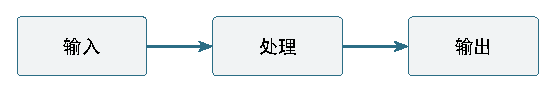
\includegraphics[width=.7\linewidth]{figures/05-pictures/demo-flow}
  \caption{数据流示意}
  \label{fig:00-flow}                % 图的标签
\end{figure}

引用时写成：见\cref{sec:00-pictures}、见\cref{fig:00-flow}。
\end{lstlisting}

效果：见\cref{sec:00-pictures}、见\cref{fig:00-flow}。表格、公式、代码清单
也一样：\cref{tab:00-compare}、\cref{eq:00-speedup}、\cref{lst:00-bubble}。
章节也可以引用，例如\cref{ch:00-guide}。

标签命名沿用"类型:章-节-序号"：\texttt{ch:} 章、\texttt{sec:} 节、
\texttt{fig:} 图、\texttt{tab:} 表、\texttt{eq:} 公式、\texttt{lst:} 代码。
标签名只用英文、数字和短横线，不要用中文和空格。

\subsection{参考文献}

引用别人的书或论文分两步：先在\textbf{本章}的 \texttt{refs.bib} 里登记条目，
再在正文里引用。

写法：

\begin{lstlisting}[language=TeX]
流水线的基本概念见经典教材\citep{patterson2020}；
\citet{amdahl1967} 很早就指出串行部分会限制整体加速比；
指令集规范这类文档同样登记成条目再引用\citep{riscvspec}。
\end{lstlisting}

效果：流水线的基本概念见经典教材 \citep{patterson2020}；
\citet{amdahl1967} 很早就指出串行部分会限制整体加速比；
指令集规范这类文档同样登记成条目再引用 \citep{riscvspec}。

\verb|\citep| 把出处放进括号，\verb|\citet| 把作者当句子成分，两种按语境挑一种。
条目本身的写法：

\begin{lstlisting}[language=TeX]
@book{patterson2020,
  author    = {Patterson, David A. and Hennessy, John L.},
  title     = {Computer Organization and Design},
  edition   = {RISC-V},
  publisher = {Morgan Kaufmann},
  year      = {2020},
}
\end{lstlisting}

三条纪律：

\begin{enumerate}
  \item 条目加在\textbf{自己章}的 \texttt{refs.bib} 里，不要去改别的章的文件；
  \item \textbf{引用键在全書范围内必须唯一}。同一本书被两章引用时，只在其中一章登记，
        另一章直接写同一个键即可——上面引用的 \texttt{patterson2020} 就登记在第 1 章，
        本章直接引用它。重复登记会让编译直接失败（BibTeX 报 \texttt{Repeated entry}）；
  \item 书末的参考文献表由各章 \texttt{refs.bib} 自动汇总，不用手工维护；
  \item 图书要写版次，网页和规范类要注明访问日期。
\end{enumerate}

\section{提示框与强调}
\label{sec:00-boxes}

\subsection{要点框}

需要把一小段话单独拎出来提醒读者时，用 \verb|\KeyPoint{标题}{说明}|。
它不加框线，靠颜色和字号区分，不会打断阅读节奏。

写法：

\begin{lstlisting}[language=TeX]
\KeyPoint{安全边界}{没有把握的结论不要写成事实，
用"待补充"占位并注明来源，等实验数据出来再补。}
\end{lstlisting}

效果：

\KeyPoint{安全边界}{没有把握的结论不要写成事实，用"待补充"占位并注明来源，
等实验数据出来再补。}

常见用法有两种：一节开头用它点出"这一节解决什么问题"，或者一段关键结论后面
用它补一句提醒。\textbf{一页里最多一两个}，多了就不"要点"了。

\subsection{其他强调手段}

\begin{description}
  \item[加粗] \verb|\textbf{...}|，用于术语第一次出现和关键结论
  \item[强调色] \verb|\textcolor{Accent}{...}|，用于需要视觉引导的关键词
  \item[缩小字号] \verb|{\small ...}|，用于附注性的补充说明
  \item[引用块] \texttt{quote} 环境，用于成段引文或需要独立成段的话
\end{description}

\subsection{一节的实验怎么排}

仓库目前没有专门的"实验"环境，约定用固定四段式：目标、环境、步骤、验收。
步骤用有序列表，验收用可勾选清单：

\begin{lstlisting}[language=TeX]
\textbf{实验目标}\quad 在 FPGA 上点亮流水线各级的指示灯。

\textbf{实验环境}\quad Vivado 2024.1；开发板型号见 config/hardware.tex。

\textbf{实验步骤}
\begin{enumerate}
  \item 综合并生成比特流；
  \item 下载到开发板；
  \item 观察指示灯的流水效果。
\end{enumerate}

\textbf{验收清单}
\begin{itemize}
  \item[$\square$] 综合没有关键警告
  \item[$\boxtimes$] 指示灯按预期流水点亮
\end{itemize}
\end{lstlisting}

如果你觉得这套四段式应该固化成统一环境，\textbf{在 Issue 里提出来}，
由主编加到 \texttt{styles/} 里，不要自己在章节里拼一个。

\section{排版细节}
\label{sec:00-details}

\subsection{字号}

正文有统一的基础字号。局部想变小或变大，要在花括号里改，让作用范围只限这一段。

写法：

\begin{lstlisting}[language=TeX]
{\small 这一段用 small 字号排版，适合表格里的补充说明。}

{\footnotesize 这一段用 footnotesize 字号排版，再小就该放进脚注了。}
\end{lstlisting}

效果：

{\small 这一段用 small 字号排版，适合表格里的补充说明。}

{\footnotesize 这一段用 footnotesize 字号排版，再小就该放进脚注了。}

\textbf{忘了加花括号}，后面所有正文都会跟着变小。

\subsection{颜色}

颜色统一取自 \texttt{config/appearance.tex}，\textbf{不要在正文里写十六进制色值}：

\begin{itemize}
  \item \textcolor{Accent}{强调色 Accent}：\verb|\textcolor{Accent}{...}|
  \item \textcolor{Muted}{次要信息 Muted}：\verb|\textcolor{Muted}{...}|
  \item \ConfigValue{品牌色 Brand}：\verb|\ConfigValue{...}|
\end{itemize}

\subsection{控制分页}

各章默认另起一页，节与节接着排。需要强制另起一页时用 \verb|\clearpage|；
不希望小标题孤零零留在页尾、正文翻到下一页时，在标题前加
\verb|\Needspace{4\baselineskip}|。

\subsection{并排两块内容}

不限于图，任何两块文字都能并排：

\begin{lstlisting}[language=TeX]
\noindent
\begin{minipage}[t]{.47\linewidth}
{\bfseries 这么写的好处}\par\vspace{2pt}
{\small 结构简单、容易验证；同一条主线逐年加码，学生的代码可以一直用下去。}
\end{minipage}\hfill
\begin{minipage}[t]{.47\linewidth}
{\bfseries 要付出的代价}\par\vspace{2pt}
{\small 覆盖面大、需要多人分工；每一层都得有能跑通的实验，否则容易停在概念上。}
\end{minipage}
\end{lstlisting}

效果：

\noindent
\begin{minipage}[t]{.47\linewidth}
{\bfseries 这么写的好处}\par\vspace{2pt}
{\small 结构简单、容易验证；同一条主线逐年加码，学生的代码可以一直用下去。}
\end{minipage}\hfill
\begin{minipage}[t]{.47\linewidth}
{\bfseries 要付出的代价}\par\vspace{2pt}
{\small 覆盖面大、需要多人分工；每一层都得有能跑通的实验，否则容易停在概念上。}
\end{minipage}

\subsection{浮动位置参数}

\texttt{[htbp]} 是给排版程序的位置建议：\texttt{h} 当前位置、\texttt{t} 页顶、
\texttt{b} 页底、\texttt{p} 单独占一页。一般写 \verb|[htbp]| 就够了。
\textbf{不要用 \texttt{[H]}}——那是强制钉在当前位置，容易在页面底部留出大片空白。

\subsection{语法速查表}

\cref{tab:00-cheatsheet} 把全章用到的语法汇总在一处。它同时是 \texttt{longtable}
的实例：表格超过一页会自动断开，并在新页重复表头。

\begin{longtable}{@{}p{40mm}p{94mm}@{}}
\caption{常用语法速查表（长表自动跨页）}\label{tab:00-cheatsheet}\\
\toprule
想写什么 & 语法 \\
\midrule
\endfirsthead
\multicolumn{2}{@{}l}{{\small\itshape 续表}}\\
\toprule
想写什么 & 语法 \\
\midrule
\endhead
\bottomrule
\endlastfoot
一级标题 & \texttt{\textbackslash section\{标题\}}，一节一个文件 \\
二级标题 & \texttt{\textbackslash subsection\{标题\}} \\
三级标题 & \texttt{\textbackslash subsubsection\{标题\}} \\
加粗 / 斜体 & \texttt{\textbackslash textbf\{...\}}、\texttt{\textbackslash emph\{...\}} \\
等宽字体 & \texttt{\textbackslash texttt\{...\}}，用于文件名、命令、类型名 \\
颜色 & \texttt{\textbackslash textcolor\{Accent\}\{...\}}，或 \texttt{\textbackslash ConfigValue\{...\}} \\
脚注 & \texttt{\textbackslash footnote\{说明\}} \\
无序 / 有序 / 术语列表 & \texttt{itemize}、\texttt{enumerate}、\texttt{description} \\
引用块 & \texttt{\textbackslash begin\{quote\}} 与 \texttt{\textbackslash end\{quote\}} \\
插图 & \texttt{\textbackslash includegraphics[width=.7\textbackslash linewidth]\{路径\}} \\
图题与标签 & \texttt{\textbackslash caption\{...\}} 加 \texttt{\textbackslash label\{fig:...\}} \\
三线表 & \texttt{tabular} 加 \texttt{\textbackslash toprule} / \texttt{\textbackslash midrule} / \texttt{\textbackslash bottomrule} \\
自适应宽表 & \texttt{\textbackslash begin\{tabularx\}\{\textbackslash linewidth\}\{...\}} \\
跨页长表 & \texttt{\textbackslash begin\{longtable\}}，本表就是实例 \\
代码清单 & \texttt{\textbackslash CodeListing\{code/节/文件\}\{题注\}} \\
指定语言的代码 & \texttt{\textbackslash CodeListing[Verilog]\{...\}\{...\}} \\
带标签的代码 & \texttt{\textbackslash lstinputlisting[...label=\{lst:...\}]\{...\}} \\
行内代码 & \texttt{\textbackslash lstinline} 或 \texttt{\textbackslash verb} \\
行内公式 & \texttt{\$T = 1/f\$} \\
编号公式 & \texttt{\textbackslash begin\{equation\}} 加 \texttt{\textbackslash label\{eq:...\}} \\
多行公式 & \texttt{\textbackslash begin\{align\}}，用 \texttt{\&} 对齐等号 \\
定义 / 定理 / 例题 / 证明 & \texttt{definition}、\texttt{theorem}、\texttt{example}、\texttt{proof} 环境 \\
交叉引用 & \texttt{\textbackslash cref\{标签\}} \\
引用文献 & \texttt{\textbackslash citep\{键\}} 与 \texttt{\textbackslash citet\{键\}} \\
要点框 & \texttt{\textbackslash KeyPoint\{标题\}\{说明\}} \\
强制分页 & \texttt{\textbackslash clearpage} \\
\end{longtable}

\subsection{常见错误清单}

\begin{enumerate}
  \item \textbf{手打章节号、图表号}。要写成 \verb|\cref{...}|，手打的数字改一次就错。
  \item \textbf{用 \texttt{\textbackslash\textbackslash} 换行}。段落之间空一行即可。
  \item \textbf{把长代码贴进正文}。放到 \texttt{code/} 下，用 \verb|\CodeListing| 引入。
  \item \textbf{在正文里硬写字号、颜色、间距}。这类全局参数统一放
        \texttt{config/appearance.tex}。
  \item \textbf{修改生成文件}。\texttt{config/manifest.tex} 与 \texttt{config/README.md}
        由脚本生成，手工改了下次会被覆盖。
  \item \textbf{顺手改别人的章}。只动自己负责的目录；需要跨章改动先在 Issue 里说一声。
  \item \textbf{图片或代码路径写错}。章里的路径相对本章目录，例如
        \texttt{figures/\allowbreak05-pictures/\allowbreak demo-flow}，
        不要写成仓库根目录下的路径。
  \item \textbf{引用前忘了登记文献}。先在 \texttt{refs.bib} 里加条目，再写 \verb|\citep|。
  \item \textbf{把编译产物提交上去}。\texttt{.aux}、\texttt{.log}、\texttt{.pdf} 都已被
        \texttt{.gitignore} 忽略，\texttt{git status} 里看不到它们属正常。
  \item \textbf{中英文之间手敲空格}。样式会自动处理间距，手敲反而会让断行位置变怪。
\end{enumerate}

\subsection{交付前的检查清单}

\begin{enumerate}
  \item 跑一遍 \verb|scripts/build.sh|，确认 \texttt{build/main.log} 里没有以
        \texttt{!} 开头的错误；
  \item 搜一遍 \texttt{待补充} 和 \texttt{TODO}，确认本节该填的占位都填完了；
  \item 确认每张图、每个表、每个公式都在正文里被引用过，不留"孤儿"；
  \item 在日志里搜 \texttt{undefined}，确认没有未解析的引用与引文；
  \item 在任务 Issue 下评论 \verb|/complete| 发起复核。
\end{enumerate}

\section{素材放哪里}
\label{sec:00-assets}

图片和代码按"越专用越靠近正文"放，路径\textbf{相对所在单元的目录}写。
本节用来演示的图就放在本节自己的目录里：

\begin{figure}[htbp]
\centering
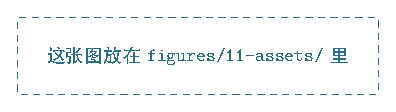
\includegraphics[width=.72\linewidth]{figures/11-assets/demo-marker}
\caption{本节专用图：放在 \texttt{figures/11-assets/} 下}
\label{fig:00-marker}
\end{figure}

\cref{fig:00-marker} 引用的是 \texttt{figures/11-assets/demo-marker}，
路径里没有出现 \texttt{chapters/} 或 \texttt{00-typesetting-guide/}——
因为章里的路径都相对本章目录。这样调整章节顺序时，素材会跟着章目录一起走。

三层规则如下。引用素材都写成 \verb|\includegraphics{路径}|，区别只在\textbf{路径怎么写}：

\begin{table}[htbp]
\centering
\caption{素材放在哪一层}
\label{tab:00-asset-levels}
\begin{tabularx}{\linewidth}{@{}P{22mm}P{54mm}Y@{}}
\toprule
通用程度 & 放在哪里 & 路径怎么写 \\
\midrule
本节专用 & 本章的 \texttt{figures/}、\texttt{code/} 下，
  按节文件名建子目录 & \texttt{figures/05-pictures/demo-flow} \\
本章多节共用 & 本章的 \texttt{figures/}、\texttt{code/} 根下 &
  \texttt{figures/chapter-overview} \\
跨章复用 & 放在主用它的那一章，别的章引用 & 从本章出发写
  \texttt{../NN-xxx/figures/文件名} \\
\bottomrule
\end{tabularx}
\end{table}

本章两种用法都有实例：\cref{fig:00-flow} 是第 5 节专用的图，放在
\texttt{figures/05-pictures/} 下；\cref{fig:00-marker} 是本节专用的图，
放在 \texttt{figures/11-assets/} 下。

还有几条规矩：

\begin{itemize}
  \item 文件名用小写英文加连字符，例如 \texttt{pipeline-hazard.pdf}，
        \textbf{不要用中文名和空格}——空格在某些工具里会出问题；
  \item 图片优先用矢量格式（PDF、SVG），位图用 PNG，照片用 JPG；
  \item 跨章复用的图只存一份，不要复制到多个章；用
        \texttt{../NN-xxx/figures/文件名} 引用；
  \item 前言和附录是全书级文件，由 \texttt{main.tex} 直接读入，
        引用素材时写从仓库根目录起的路径，例如 \texttt{backmatter/code/hello.c}；
  \item 每份素材注明来源与许可，第三方图片要确认可用范围。
\end{itemize}

\KeyPoint{路径记不住怎么办}{只记一句话：\textbf{路径相对你现在写的这个文件所在的单元目录}。
写的时候照着同一章其它地方的写法抄一遍，改文件名即可。}


\end{document}
